\documentclass[conference]{IEEEtran}
\renewcommand\IEEEkeywordsname{keywords}
\usepackage{graphicx}
\usepackage{epstopdf}
\usepackage{float}
\usepackage{amssymb}
\usepackage{multirow}
\usepackage[english]{babel}
\usepackage{algorithmic,algorithm}
\renewcommand{\algorithmicrequire}{\textbf{Input:}}
\renewcommand{\algorithmicensure}{\textbf{Output:}}
\usepackage{enumerate}
\usepackage{lipsum}% http://ctan.org/pkg/lipsum
\hyphenation{op-tical net-works semi-conduc-tor}
\usepackage{booktabs}
\usepackage{amsmath}
\usepackage[smallscripts]{moresize}
%\usepackage[numbers,sort&compress]{natbib}
\usepackage[numbers,sort]{natbib}
\usepackage[most]{tcolorbox}
%\usepackage{ctable}

\begin{document}

\title{Applying Convolutional Neural Networks for Image-based Disease Detection in Potato Plants}
%%%%%%%%%%%%%%%%%%%%%%%%%%%%%%%%%%%%%%%
% \author{\IEEEauthorblockN{Utpal Kant Singh, Rajnish Kumar, Saurabh Kumar, Shibasish Kar, Santos Kumar Baliarsingh}

% \IEEEauthorblockA{School of Computer Engineering,
% KIIT Deemed to be University, Bhubaneswar, 751024, India}
% \{20051117, 2005118, 20051096, 2005335, santos.baliarsinghfcs\}@kiit.ac.in
% }
%%%%%%%%%%%%%%%%%%%%%%%%%%%%%%%%%%%%
\author{\IEEEauthorblockN{Utpal Kant Singh}
\IEEEauthorblockA{School of Computer Engineering\\
KIIT Deemed to be University,\\ Bhubaneswar, India 751024\\
Email: utpalkant.4855@gmail.com}
\and
\IEEEauthorblockN{Vishal R. Satpute}
\IEEEauthorblockA{Department of Electronics and \\Communication Engineering\\
VNIT, Nagpur, India 440010\\
Email: vrsatpute@ece.vnit.ac.in}
}
%%%%%%%%%%%%%%%%%%%%%%%%%%%%%%%%%%%%%%%%%%%%%


\maketitle

\begin{abstract}

Potatoes are widely grown in India, thanks to their suitability for the country's tropical climate.The growth of potatoes, however, can be hampered by a number of variables, such as the climate, which can result in lower yields. Plant diseases can cause considerable financial losses and constitute a serious danger to agricultural output. Potato crop disease identification using conventional approaches has been shown to be inefficient and time-consuming. For the best results, early illness diagnosis is essential. This study explores the possibility of deep learning methods, particularly convolutional neural networks (CNNs), for recognising potato plant illnesses utilising computer vision technologies in order to address this difficulty. With an average illness categorization accuracy of 98\%, the research shows the effectiveness of the suggested strategy. \\

 
\end{abstract}


\begin{IEEEkeywords}
Deep Learning, Convolutional Neural Network, Machine Learning, Potato Leaf Disease Detection 
\end{IEEEkeywords}
 
\IEEEpeerreviewmaketitle



\section{Introduction}



\subsection{Motivation}
Potato farming plays a significant role in the Indian economy, as farmers cultivate various crops to meet the country's agricultural demands. However, potato plants are susceptible to diseases, which can lead to substantial losses in both yield and quality. Early detection and treatment of these diseases are crucial for farmers to protect their livelihoods. Traditional disease management methods, such as pesticide use, can have adverse effects on the environment. Therefore, early disease detection promotes sustainable agricultural practices by minimizing the reliance on chemical treatments. Certain potato diseases can also pose health risks to humans through contaminated produce or exposure to toxins. Timely detection and treatment of these diseases can help mitigate these risks. Manual inspection-based approaches for disease detection are costly and resource-intensive, highlighting the need for automated methods that are accurate and reliable in identifying potato leaf diseases. \\ 

CNNs have revolutionised the area by making substantial strides in object detection and picture categorization. How we identify and manage plant diseases may change as a result of using CNNs into disease detection. Early detection made possible by CNNs enables quick response, lowering crop losses and increasing output. CNNs provide accurate diagnoses, minimising mistakes brought on by visual examinations and lowering reliance on human specialists. Additionally, the use of CNNs in automated illness detection has the potential to drastically lower costs and turnaround times, especially in areas with limited resources. Due of its accessibility and affordability, this technology helps farmers overcome obstacles caused by a lack of resources and knowledge.\\ 

Using CNNs to identify illnesses automatically can also help reduce the cost and turnaround time associated with performing traditional disease diagnosis methods. This is essential in developing countries because there might not be enough resources or experts who are equipped to recognise and cure plant diseases. CNNs make diagnosis more affordable and accessible for farmers by reducing the cost and time involved.

\subsection{Contributions}
\begin{itemize}
    \item A system for classifying illnesses affecting potato leaves is created using a convolutional neural network (CNN) architecture based on deep learning. The system's main goal is to accurately and precisely classify the many diseases that impact potato plants.
    \item TThe CNN model, which is suggested for the classification of potato plant leaf diseases, outperforms more sophisticated models in tests and comparisons, demonstrating its exceptional efficiency.
    \item Through trials on a publicly accessible dataset of potato plant leaf diseases, the efficacy and applicability of the proposed CNN-based technique are assessed. The experimental findings provide important information on how the suggested approach to disease identification and classification in agriculture might be used in practise.\\
\end{itemize}
 
The objective of this study is to evaluate CNNs' potential for automatically spotting disease in tomato leaves. If the findings of this study were used to the creation of more accurate and efficient methods of recognising illnesses in tomato crops, farmers and the global food supply chain would benefit.


\section{Related Works}
A popular and healthy crop, potatoes are nevertheless susceptible to a number of illnesses that, if not properly diagnosed and treated, can result in significant crop output losses. To address this issue, researchers have begun automating the detection and categorization of illnesses in potato plants using deep learning techniques, specifically CNNs.\\

Early detection and effective management of potato leaf diseases are crucial for minimizing the impact. Asif et al. \cite{9316021}, a proposed model utilizing image processing methods aims to accurately identify and detect diseases in potato leaves. Among various machine learning algorithms, the Convolutional Neural Network (CNN) model is employed due to its superior performance in image classification tasks. Five different algorithms, including AlexNet, VggNet, ResNet, LeNet, and the offered Sequential model, are utilized in this study. The model is trained using both normal and disease-affected leaf images to distinguish between healthy and abnormal aspects of potato leaves. Through the implemented algorithm, the potato plant leaves are classified as either diseased or normal, achieving a remarkable precision of 97\%. There paper highlights the significance of disease detection in potato plants and emphasizes the effectiveness of the proposed CNN-based model in accurately identifying potato leaf diseases.\\


With the advancement of agricultural technology and the integration of artificial intelligence in plant disease diagnosis, it is crucial to conduct relevant research for sustainable agricultural development. Diseases such as early blight and late blight have a significant impact on the quality and quantity of potato crops, and the manual identification of these leaf diseases can be time-consuming and challenging. Efficient and automated detection of these diseases at an early stage can greatly contribute to improving potato crop production. Previous studies have proposed various models for detecting plant diseases. \cite{9121067} This paper presents a model that utilizes pre-trained models like VGG19 for fine-tuning through transfer learning to extract relevant features from the dataset. Multiple classifiers are employed, and logistic regression demonstrates superior performance with a classification accuracy of 97.8\% on the test dataset. \cite{9121067}This research contributes to the development of efficient disease detection systems for potatoes, aiding in the improvement of crop productivity and quality.\\

In their study, Hari et al\cite{8899748}, introduced the Plant Disease Detection Neural Network (PDDNN), a unique CNN model for analysing leaf pictures of diverse crops. The 16-layer PDDNN incorporates several filters, dropout layers, and max pool layers to enhance performance. The PDDNN obtained an amazing accuracy rate of 86\% using an enlarged dataset of 14,810 pictures. Its higher performance was demonstrated by the fact that it outperformed the Mobilenet 50 network's accuracy by about 7\%.\\

Potato diseases pose a major threat to the quality and quantity of potato harvests. Late detection and incorrect classification of diseases can exacerbate plant conditions, leading to substantial losses. Leaf conditions provide valuable insights for identifying various diseases in potato plants. \cite{9231784} This research presents a system for accurately classifying four types of potato plant diseases based on leaf conditions. Deep learning techniques using the VGG16 and VGG19 convolutional neural network architectures are employed to develop a classification system. The experimental results demonstrate an average accuracy of 91\%, indicating the effectiveness of the deep neural network approach in potato disease classification. This study contributes to the field by providing a reliable and accurate method for early disease detection, enabling timely intervention and improved crop management.\\

Existing machine learning methods often struggle to generalize across different crop species and diseases, as they are trained and tested on specific regional datasets. In this research \cite{electronics10172064}, a multi-level deep learning model is proposed for the recognition of potato leaf diseases. The model incorporates YOLOv5 image segmentation to extract potato leaves from plant images, followed by a novel convolutional neural network for detecting early blight and late blight diseases from potato leaf images. The model is trained and evaluated on a dataset comprising 4062 images collected from the Central Punjab region of Pakistan, achieving an impressive accuracy of 99.75\%. Furthermore, the model's performance is compared to state-of-the-art approaches and demonstrates superior accuracy and computational efficiency. \cite{electronics10172064} This research contributes to the advancement of potato leaf disease detection, offering a robust and accurate solution for early diagnosis and effective management of potato crops. \\

Effective control and management of potato leaf diseases are essential for increasing production and minimizing losses for farmers. Automating the identification of infected crops can greatly assist farmers in disease control. \cite{9181312} This research proposes a Convolutional Neural Network (CNN) architecture specifically designed for potato disease detection. A training dataset is created through image processing techniques in the CNN framework. The Adam optimizer and cross entropy analysis are utilized, with softmax serving as the final judgment function. The architecture is optimized to minimize resource usage while maintaining high accuracy. Experimental results demonstrate the effectiveness of the proposed model, achieving a disease judgment accuracy of 99\% with a parameter usage of 10,089,219. This study contributes to the field by providing a robust and accurate approach for potato disease detection, enabling timely intervention and improved disease management practices.\\

Afonso et al. \cite{AFONSO20196} explores the application of deep learning methods for detecting blackleg diseased potato plants. Two deep convolutional neural networks, including ResNet18, are trained on RGB images containing both healthy and diseased plants. Experimental results demonstrate the effectiveness of the ResNet18 network, achieving a precision of 95\% and recall of 91\% for the disease class. These findings highlight the potential of convolutional neural networks as a valuable tool for detecting blackleg diseased potato plants, enabling early intervention and improved disease management strategies.\\

 Deep learning-based computer vision techniques, including Convolutional Neural Networks (CNN), have been applied to identify plant diseases. This paper \cite{sharma2022plant} proposes a CNN model for classifying rice and potato leaf diseases. The dataset includes images of rice leaves with bacterial blight, blast, brown spot, and tungro diseases, as well as potato leaf images with healthy leaves, early blight, and late blight diseases. The proposed CNN model achieved high accuracy, with 99.58\% for rice leaf classification and 97.66\% for potato leaf classification. The results demonstrate the superiority of the CNN model over other machine learning classifiers like Support Vector Machine, K-Nearest Neighbors, Decision Tree, and Random Forest in image classification tasks for plant disease identification.\\

Automating disease diagnosis has become essential to modernize the potato industry and mitigate the impact of diseases on crop yield. Early detection and intervention can prevent substantial economic losses. \cite{10080063} This study proposes a new model for accurately identifying and detecting potato leaf diseases using image processing techniques. The Convolutional Neural Network (CNN) model is utilized to classify diseases in potato leaf images, achieving a model accuracy of 94.2\%. The model is trained and tested on both healthy and diseased potato leaves, enabling the distinction between the two. The algorithm provides a classification of the potato leaf as either healthy or unhealthy, offering a reliable tool for disease detection in the potato farming sector.\\

The potato is a globally significant food crop, and its cultivation has gained remarkable popularity in Bangladesh in recent decades. However, the growth of potato plants is hindered by various diseases, particularly those affecting the leaves, such as Early Blight (EB) and Late Blight (LB). Early detection of these diseases is crucial for enhancing crop production. To address this issue, image processing techniques combined with machine learning are proposed in this paper \cite{9198563} to automatically identify and classify potato leaf diseases. The study utilizes a dataset of 450 images of healthy and diseased potato leaves obtained from the publicly available Plant Village database. Seven classifier algorithms are employed to recognize and classify the health status of leaves, with the Random Forest classifier achieving an impressive accuracy of 97\%. This approach offers a promising solution for the automatic detection and management of potato leaf diseases, contributing to improved crop production.\\

Potato leaf diseases pose significant challenges for potato farmers worldwide, impacting crop quality and yield. Early detection and effective management of these diseases are crucial to minimize financial losses.\cite{10112080} This research proposes a novel approach using image processing techniques to accurately identify and diagnose potato leaf diseases. The utilization of Convolutional Neural Networks (CNN), a powerful machine learning algorithm, for image classification demonstrates superior performance compared to other methods. By distinguishing between normal and disease-affected potato leaves, the model achieves a high precision rate with 97\% accuracy. The implementation of this technology has the potential to greatly benefit potato farmers, reducing economic losses and enhancing disease detection efficiency in potato crops. \\


In conclusion, the use of convolutional neural networks (CNNs) has demonstrated encouraging outcomes in the automatic identification and categorization of illnesses in potato plant leaves. Numerous studies have attained notable degrees of accuracy, demonstrating the method's potential. By using methods like transfer learning, SVM classifiers, and new visual information, ongoing research intends to improve CNN performance. These improvements in the CNN-based categorization of potato leaf diseases have the potential to have a major impact on crop management practises and reduce disease-related losses.


% \begin{itemize}
%   \item \textit{Map phase}: In this phase, the input data is processed locally and an input key-value pair is created. A map function is applied to the local data by each node and consequently, the output is sent to a temporary storage with a key-value pair.
% \end{itemize}


% \begin{itemize}
%   \item \textit{Reduce phase}: This phase is carried out in three phases namely, fetch, sort, and reduce. In the first phase, it fetches local copies of all the assigned map results from the map worker nodes. In the sort phase, it merges the copied results into a single sorted set of key-value pairs. In the last phase, the reduce method is invoked for each key, with  records combined into an iterable collection. Then the final result is written and saved to the output destination HDFS. 
% \end{itemize}   
% Figure~\ref{fig:hadoop} shows the architecture and life cycle of MapReduce.




% \begin{figure*}
% \centering
% \includegraphics[width=\textwidth{flowchart2}
% \caption{The flow diagram of the proposed anomaly detection approach}
% \label{fig:architecture}
% \end{figure*}



\section{Proposed Work}
In order to identify and categorise diseases that damage potato leaves, convolutional neural networks (CNNs) would be employed in the proposed study. Given the high susceptibility of potato plants to various diseases, crop yield might be drastically decreased if the diseases are adequately detected and treated. The objectivity, timeliness, and error-proneness of conventional methods, which rely on manual inspection by experts, are constrained. Therefore, there is a need for automated systems that can detect potato leaf diseases with greater accuracy and efficacy simply looking at pictures of the leaves.

The recommended model offers a number of advantages over previous approaches used to the same purpose. It increases the ability to extract important information from images of potato leaves by applying cutting-edge techniques like transfer learning and data augmentation as well as complex CNN architectures. As a result, diseases are categorised more accurately, and the possibility of making a mistaken diagnosis is diminished.

The proposed model further overcomes the shortcomings of prior models by making use of a bigger and more varied set of potato leaf image data. The model's capacity to generalise to novel, unexplored data is enhanced by its capacity to learn a larger variety of sickness patterns. As a result, the model performs better in circumstances that it has never encountered before.

A key component of the suggested model is its efficient use of computational resources. The model uses optimised CNN architectures and methods to offer astounding accuracy while reducing processing requirements and inference time. This makes it particularly effective in contexts with limited resources for real-time applications for sickness detection and categorization.

In comparison to present models, the recommended model is often more precise, durable, and useful. In order to prevent crop losses and ensure the stability of potato production, it offers a practical way for the automated diagnosis of potato leaf diseases. This technology enables prompt reaction and efficient management strategies.

The dataset is divided into different sets for training and testing, as shown in Figure~\ref{fig: Figure 1}. For purposes of validation, a portion of the testing set is created. After being trained using the training data, the model is improved by changing its hyperparameters in accordance with the validation data. The training process is completed when the required number of epochs has been reached. Finally, the performance and effectiveness of the model are assessed using test data.

\begin{figure}[H]
 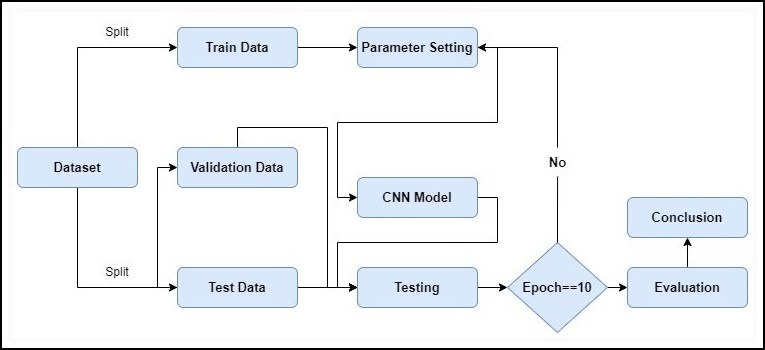
\includegraphics[width=8.8cm, height=4cm]{Tomato Final Flowchart.jpg}
\caption{Flowchart of the proposed work}
\label{fig: Figure 1}
\end{figure}

\subsection{Data Pre-Processing}
The PlantVillage dataset already contains pre-processed images with little to no distortion, so there is not a significant need for additional work to normalise the images.\\
Additionally, data augmentation techniques like rotation, flipping, and zooming were used on the training set to increase the dataset size and increase the robustness of the CNN model.\\
Overall, the information used in this endeavour to categorise potato leaf disorders is substantial, diverse, and representative of numerous potato diseases.




% \subsection{Temporal Attention module}
% Inspired by the various attention techniques~\cite{.....}, we employ a temporal attention module to capture temporal dependencies among snippets. After that, the attention scores are multiplied with the feature vectors to detect anomaly events. Thus, the temporal attention module allows the network to concentrate on the more important snippets.


\subsection{CNN - Convolutional Neural Network}

An advanced form of neural network known as a convolutional neural network (CNN) is created primarily for processing visual input like photos and videos. Due to their several layers, they have proven incredibly useful in jobs involving image and video processing. Convolutional layers in the model use trainable filters to extract important data from input photos. To decrease computational complexity, pooling layers downsample these obtained characteristics. By mapping the retrieved characteristics to the appropriate output classes, fully linked layers are used to properly categorise the input. With its use in object identification, semantic segmentation, and picture classification, CNNs have transformed computer vision. Utilising CNNs to automatically identify and categorise plant diseases, particularly those that impact tomato leaves, has been the subject of recent study. Customised variants of the ResNet architecture have been shown to be the most accurate when compared to well-known deep learning architectures like AlexNet and GoogleNet.\\

The ResNet50 architecture, initially proposed by Zhang et al. in a 2015 study \cite{Zhang_2021_WACV}, served as the foundation for our deep neural network model.

ResNet's key idea is the incorporation of residual connections, which enable information to transit across various levels and move fluidly throughout the network. This is achieved by establishing skip connections, which promote a more effective information flow by connecting the input of one layer to the output of another, creating a shortcut.\\

By utilising skip connections, ResNet successfully overcomes the problem of disappearing gradients frequently experienced in deep neural networks. These connections allow for more uniform gradient flow during backpropagation, which enhances the efficiency of deep network training. As a result, ResNet makes it possible to train very deep networks more effectively and with better gradient propagation.\\

ResNet is available in several varieties, and one of the most well-known forms is ResNet50, which has 50 layers. ResNet50's outstanding performance in tasks including scene segmentation, object tracking, and picture identification has helped it become well-known in the field of visual computing. It has raised the bar and established new norms in various fields.

\section{Experiment}
\subsection{Dataset}
The study used the publicly accessible PlantVillage dataset, which contains 54,000 labelled photos from 14 distinct crop kinds. There were 2,152 potato leaf photographs in all, with each shot measuring 256 by 256 pixels. Three classes were created from the photos of potato leaves, with one class representing healthy leaves and the other two classes reflecting varied disease states. The dataset was split into three subsets for easier analysis: the training set, which contained 70\% of the photographs; the test set, which contained 15\% of the images; and the validation set, which also contained 15\% of the images. As shown in the Figure~\ref{fig: Figure 2}, each picture in the dataset was recorded in the JPEG format and represented using the RGB colour space.

 \begin{figure}[H]
 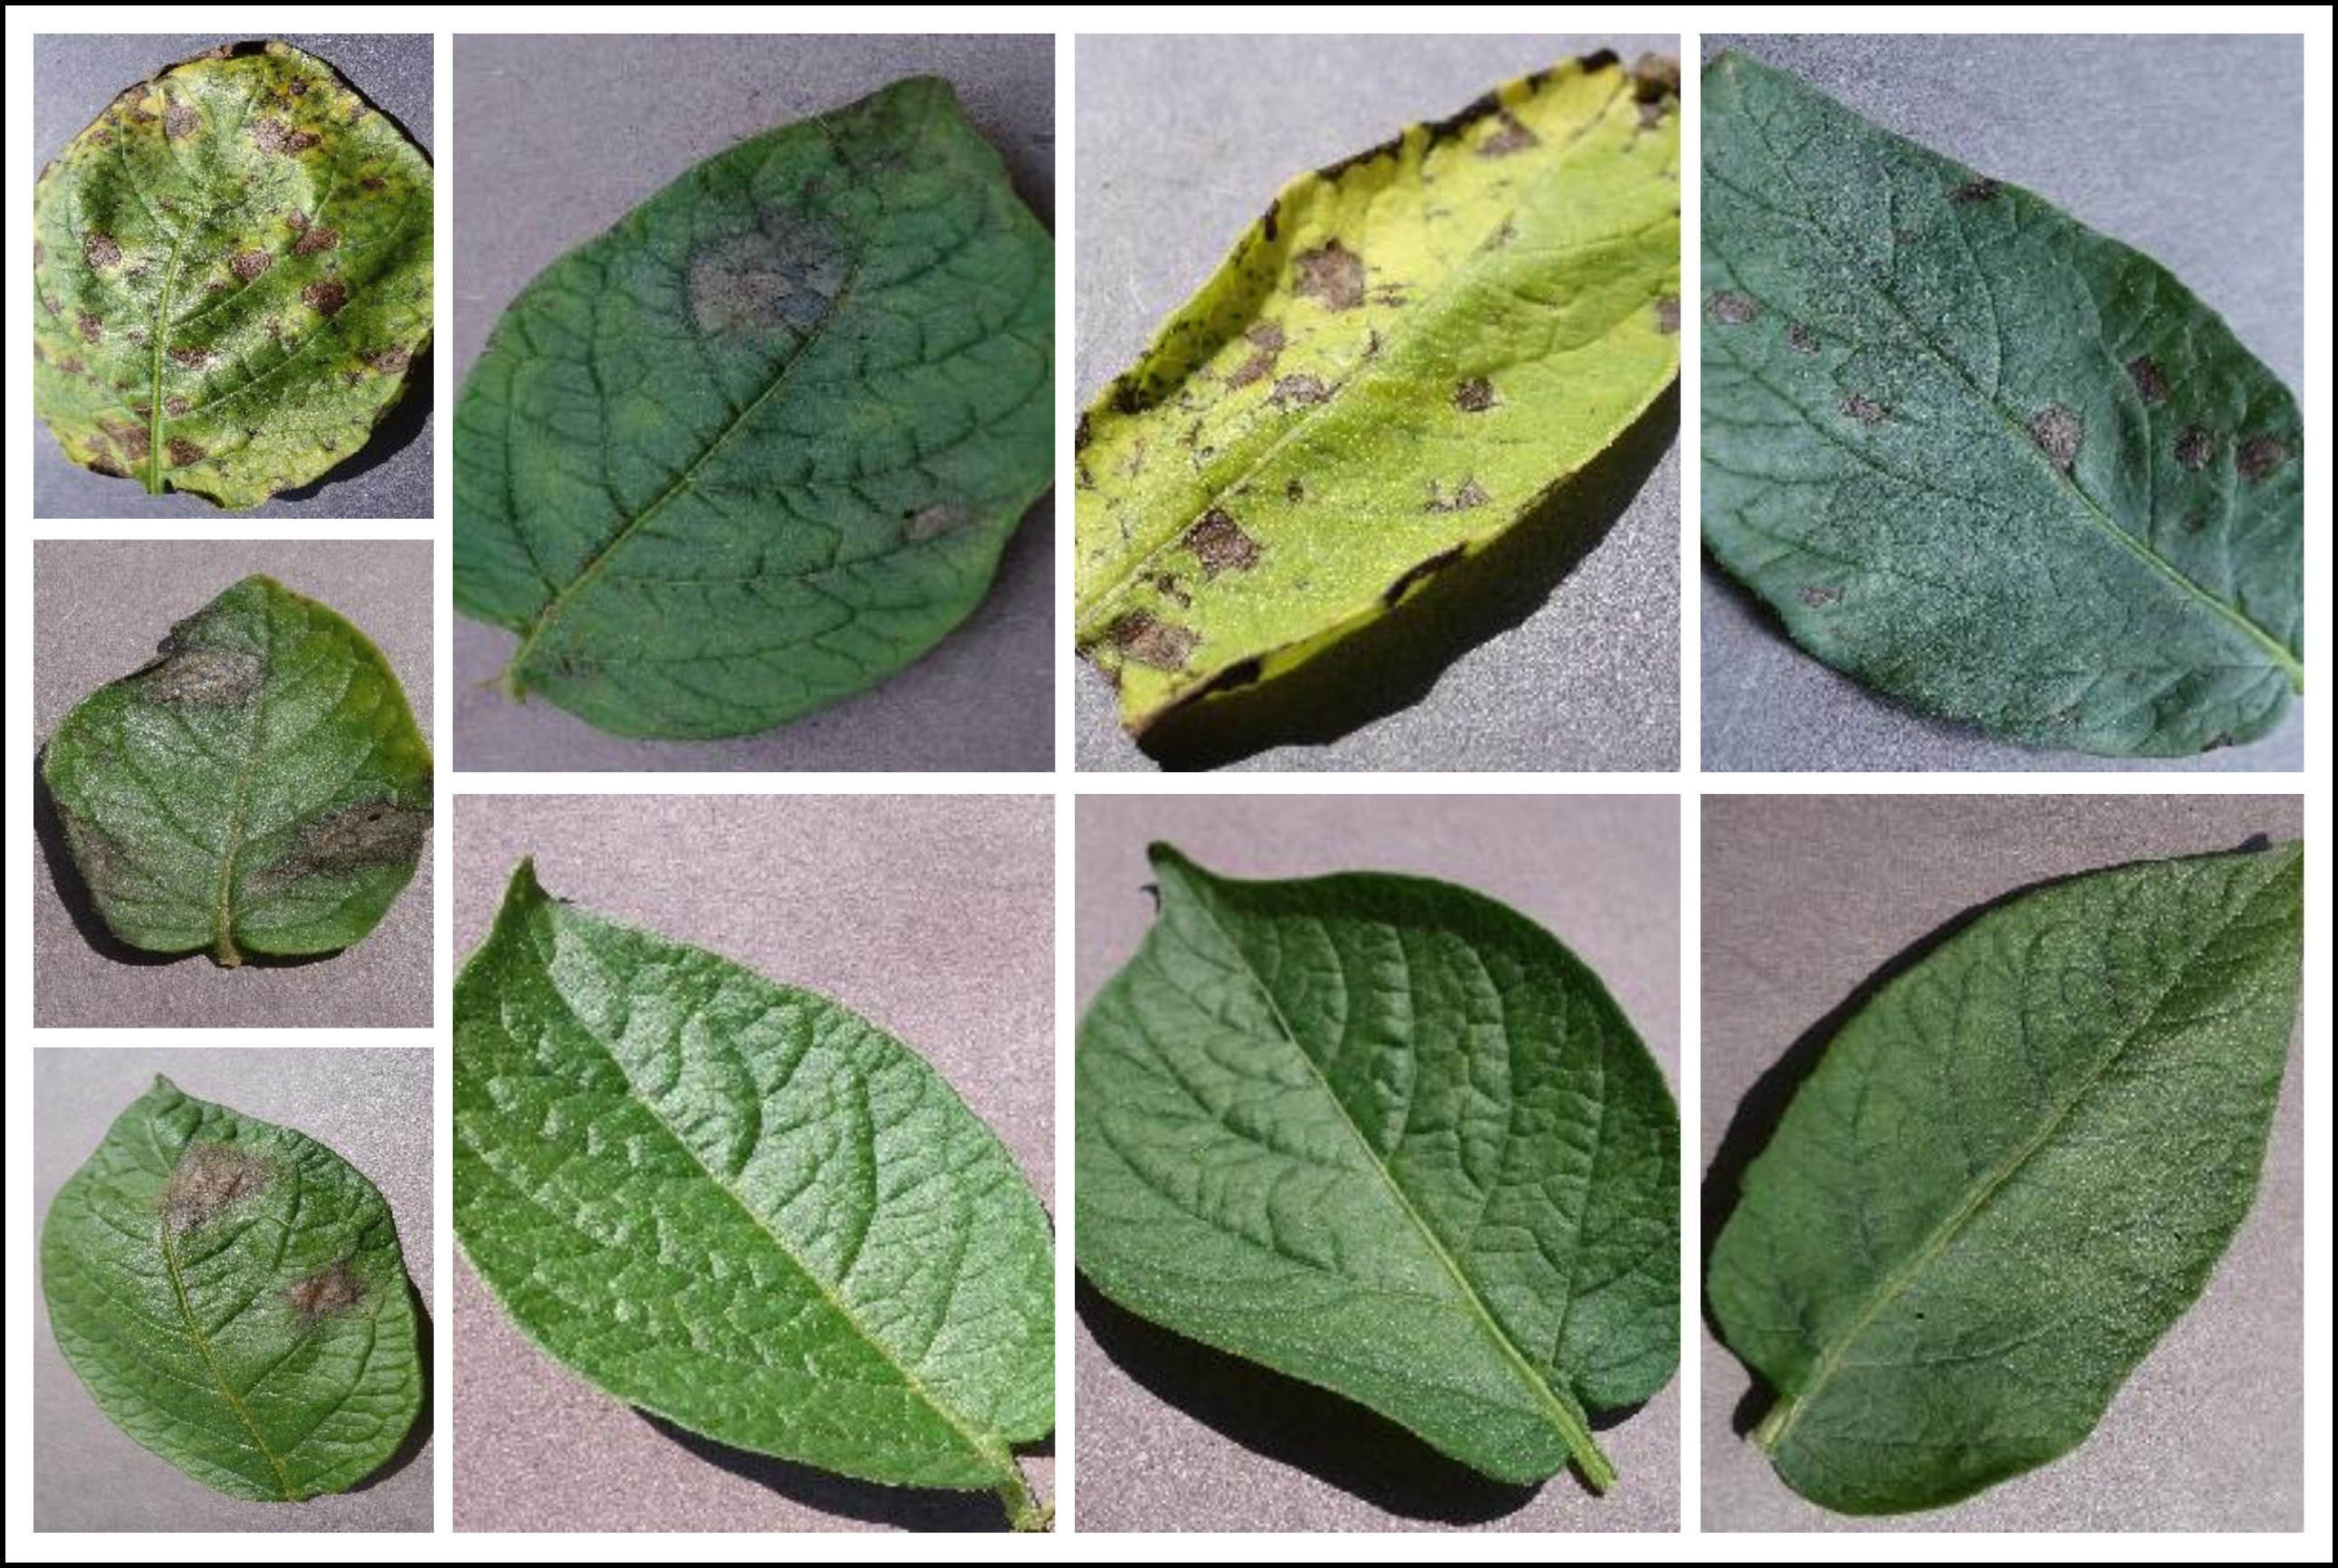
\includegraphics[width=8.8cm, height=5cm]{Potato Dataset.jpg}
\caption{Images from the datasets used}
\label{fig: Figure 2}
\end{figure}
 
\subsection{Evaluation Measure}
Several assessment metrics, with classification accuracy as the main indicator, were employed to determine how well the suggested CNN model performed in diagnosing potato leaf diseases. This statistic calculates the proportion of photos in the test set that were properly identified when compared to all of the photographs.\\ 


A number of measures, such as recall, precision, and F1-score, are used to evaluate the effectiveness of the proposed model in addition to accuracy. The relationship between successfully predicted positive cases and all projected positive instances is measured by precision, whereas the relationship between effectively anticipated positive occurrences and all actual positive instances is measured by recall. The harmonic mean of accuracy and recall is calculated using the F1-score, a detailed statistic.\
The proposed CNN model's ability to identify between potato leaf diseases may generally be evaluated using a combination of these assessment metrics, which can also be used to compare the proposed CNN model to other models that are already in use.


\subsection{Experiment setting} 
Python programming language and a number of libraries, including as TensorFlow, Keras, and OpenCV, are used to create the proposed CNN model for detecting leaf illnesses in potato plants. An i7-6800 processor running at 3.4 GHz, a 2 GB NVIDIA GeForce GPU, and 16 GB of RAM power the computer system used to run the model. A learning rate of 0.001 and a batch size of 32 are used throughout the course of 10 epochs to train the model using the Adaptive Moment Estimation optimizer. A training set, a validation set, and a testing set, each with relative proportions of 70\%, 15\%, and 15\%, are created from the collection of potato leaf pictures.

\section{Results and Discussion}
% In this section, we present and discuss the experimental results obtained 

Several measures, including the F1-score, recall, accuracy, precision, and confusion matrix, were used to assess the model's efficacy. The greatest validation accuracy attained was 94.7\%, whereas the claimed training accuracy was 97.8\%. The model performed classification tasks well on average, with a validation accuracy of 98\%.


 \begin{figure}[H]
 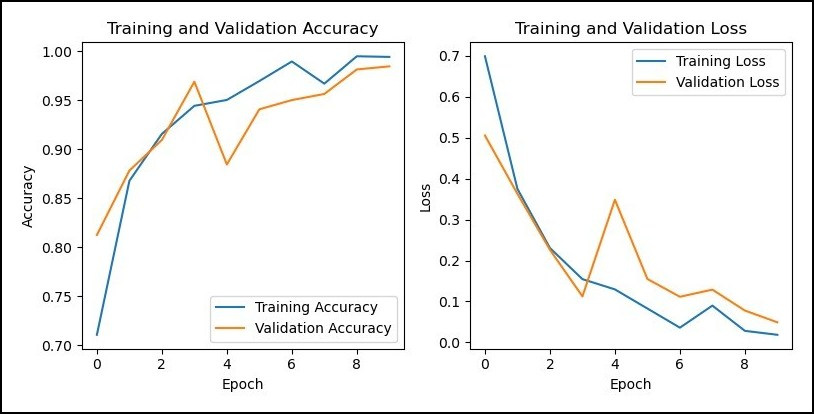
\includegraphics[width=8.9cm, height=4.5cm]{Potato Accuracy and Loss.jpg}
\caption{The model's accuracy  and loss was assessed during both the training and validation stages.}
\label{fig: Figure 3}
\end{figure}
Visually, the graphs display the model's accuracy and loss. The accuracy graph, as shown in Figure~\ref{fig: Figure 3}, showed a steady increase in accuracy before stabilising, while the loss graph revealed a gradual decrease in loss before doing the same. The performance of the model is demonstrated by these graphs, which also demonstrate that it is a valuable tool for categorising the 10 different kinds of tomato leaf diseases. These graphs improve our comprehension of the model's capabilities and reaffirm its significance as a trustworthy tool for illness categorization by offering a clear visual of the model's development.


 \begin{figure}[H]
 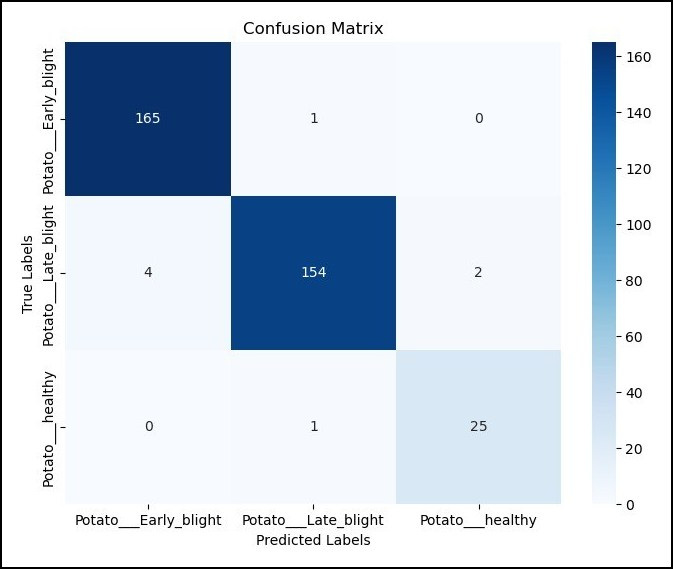
\includegraphics[width=8.8cm, height=5cm]{Potato Confusion Matrix.jpg}
\caption{Confusion matrix for the model used in the paper}
\label{fig: Figure 4}
\end{figure}

 \begin{figure}[H]
 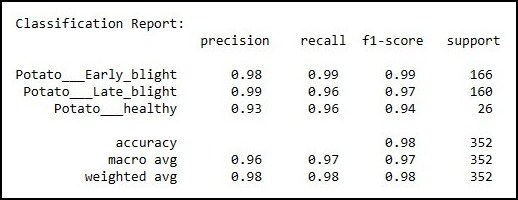
\includegraphics[width=8.8cm, height=4cm]{Potato Stats.jpg}
\caption{Accuracy, Precision, Recall and F1-Score for the used model}
\label{fig: Figure 5}
\end{figure}

With the use of the confusion matrix and many performance indicators, such as accuracy, precision, recall, and F1 score, we thoroughly assessed image classification models. By contrasting the predicted labels with the actual labels, the confusion matrix allowed us to visually assess how well the model performed. The accuracy, which gauges the classification's overall accuracy, was determined using the confusion matrix. The F1 score also took into account the model's balance between precision and recall, which is displayed in the figure figure~\ref{fig: Figure 4} and figure~\ref{fig: Figure 5}. Precision assessed the model's capacity to accurately identify positive cases, recall assessed its ability to capture all positive occurrences.
  
\section{Conclusion and Future Work}
A large amount of the population in India is supported by the agricultural industry, and crop disease detection is essential to the sector's expansion and sustainability. Similar to tomato plants, potato plants can contract a number of illnesses that can limit their ability to develop and produce. In this study, a convolutional neural network (CNN) model is used to suggest a simple method for categorising and diagnosing illnesses affecting potato leaves. The Plant Village dataset was used for this. The programme can make precise predictions by examining patterns and traits in photos of leaves. The performance and resilience of the model are improved by the use of data augmentation approaches. The suggested method achieves a noteworthy accuracy rate of 95–98\% while using a small amount of processing power. In order to enhance the performance of the model even further, future research can concentrate on investigating other optimizers, learning rates, and fresher designs. Further improvements can result by optimising the training parameters to cut training timeframes. The application of this method extends beyond potatoes and may be modified for disease detection in other plants, such as apples, brinjal and cucumbers.

% \section*{Acknowledgment}
% This work is supported by the FIST project of Department of Science and Technology, Govt. of India. We thank Mr. xxxxxxxxxxxxxxxxxx for his assistance with language editing, and proofreading. 
%\section{References}
\bibliographystyle{IEEEtran}
\bibliography{santos_bib}

\end{document}







